\documentclass[11pt]{amsart}          
\usepackage[a4paper,verbose]{geometry}
\geometry{top=3cm,bottom=3cm,left=3cm,right=3cm,textheight=595pt}
\setlength{\parskip}{0.3em}
% ==============================
% PACKAGES
% ==============================

\usepackage{amsfonts}
\usepackage{amssymb}  
\usepackage{amsthm} 
\usepackage{amsmath} 
\usepackage{caption}
\usepackage[inline]{enumitem}
\setlist{itemsep=0em, topsep=0em, parsep=0em}
\setlist[enumerate]{label=(\alph*)}
\usepackage{etoolbox}
\usepackage{stmaryrd} 
\usepackage[dvipsnames]{xcolor}
\usepackage[]{hyperref}
\hypersetup{
  colorlinks,
  linkcolor=blue,
  citecolor=blue,
  urlcolor=blue}
\usepackage{graphicx}
\graphicspath{{assets/}}
\usepackage{mathtools}

\usepackage{tikz-cd}
\usepackage{minted}
\usepackage{float}
\usetikzlibrary{
  matrix,
  arrows,
  shapes
}

\setcounter{tocdepth}{1} % Sets depth for table of contents. 

% ======================================
% MACROS
%
% Add your own macros below here
% ======================================

\newcommand{\rr}{{\mathbb{R}}}
\newcommand{\nn}{{\mathbb{N}}}
\newcommand{\iso}{\cong}
\newcommand{\too}{\longrightarrow}
\newcommand{\tto}{\rightrightarrows}
\newcommand{\To}[1]{\xrightarrow{#1}}
\newcommand{\Too}[1]{\To{\;\;#1\;\;}}
\newcommand{\from}{\leftarrow}
\newcommand{\From}[1]{\xleftarrow{#1}}
\newcommand{\Cat}[1]{\mathbf{#1}}
\newcommand{\cat}[1]{\mathcal{#1}}
\newtheorem*{remark}{Remark}
\renewcommand{\ss}{\subseteq}
\newcommand{\hask}[1]{\mintinline{Haskell}{#1}}
\newenvironment{haskell}
  {\VerbatimEnvironment
  	\begin{minted}[escapeinside=??, mathescape=true,frame=single, framesep=5pt, tabsize=1]{Haskell}}
  {\end{minted}}

% ======================================
% FRONT MATTER
% ======================================

\author{Bartosz Milewski}
\title{Fixed Points of Endofunctors}

\begin{document}
\maketitle{}

\href{https://github.com/BartoszMilewski/Publications/blob/master/Algebras2.pdf}{Previously}, we've been discussing the construction of initial algebras and terminal coalgebras in terms of colimits and limits. By Lambek's lemma, both constructions lead to fixed points of the functor in question (the least one and the greatest one, respectively). ln this installment we'll dig into alternative definitions of these (co-)algebras, first in Haskell, to build some intuition, and then using (co-)end calculus in category theory.

\section{Initial algebra and catamorphisms}

The initial algebra for a given functor \hask{f} is defined by its universal property. Take any other algebra with the carrier \hask{a} and the structure map \hask{f a -> a}. There must exist a unique algebra morphism from the initial algebra to it. Let's call the carrier for the initial algebra \hask{Mu f}. The unique morphism is given by the catamorphism, with the following signature
\begin{haskell}
cata :: Functor f => (f a -> a) -> (Mu f -> a)
\end{haskell}
or, after rearranging the arguments,
\begin{haskell}
cata :: Functor f => Mu f -> (f a -> a) -> a
\end{haskell}

This universal property can be used in the definition of \hask{Mu f} 
\begin{haskell}
newtype Mu f = Mu (forall a. (f a -> a) -> a)
\end{haskell}
A value of this type is a polymorphic function. This function, for any type \hask{a} and any function \hask{f a -> a}, will produce a value of type \hask{a}. In other words, it's a \emph{gigantic product} of all possible catamorphisms. 

Notice that this definition requires the following language pragma
\begin{haskell}
{-# language RankNTypes #-}
\end{haskell}

This is an example of a definition in terms of the \emph{mapping out} property. An object is uniquely defined by the outgoing morphisms to all other objects. This is the consequence of the Yoneda lemma.

It's easy to define a catamorphism in terms of \hask{Mu}
\begin{haskell}
cataMu :: Functor f => Algebra f a -> Mu f -> a
cataMu alg (Mu cata) = cata alg
\end{haskell}
This is because \hask{Mu} is a polymorphic catamorphism, and the compiler will automatically instantiate it for the proper type.

The definition of \hask{Mu f} is workable, if a bit unwieldy---the challenge is to construct terms of type \hask{Mu f}. I'll show you how to do it using a list as an example. We'll convert a list of \hask{a} to a term of type \hask{Mu (ListF a)}. 

As a reminder, the functor \hask{ListF a} is defined as
\begin{haskell}
data ListF a x = NilF | ConsF a x
\end{haskell}
In essence, if we can provide the implementation of all possible folds for a given list, we have defined the list. This is a little like defining a function by specifying its integrals with all possible test functions (that's how distributions are defined in calculus).
\begin{haskell}
fromList :: [a] -> Mu (ListF a)
fromList as = Mu (\alg -> go alg as)
  where go alg [] = alg NilF
        go alg (n: ns) = alg (ConsF n (go alg ns))
\end{haskell}
You can now verify that
\begin{haskell}
cataMu sumAlg (fromList [1..10])
\end{haskell}
produces the correct result for the following algebra
\begin{haskell}
sumAlg :: Algebra (ListF Int) Int
sumAlg NilF = 0
sumAlg (ConsF a x) = a + x
\end{haskell}

\section{Terminal coalgebra and anamorphisms}

The terminal coalgebra, on the other hand, is defined by its \emph{mapping in} property. We start by looking at the signature of the anamorphism. \hask{Nu f} is the terminal coalgebra
\begin{haskell}
ana :: Functor f => (a -> f a) -> (a -> Nu f)
\end{haskell}
We can uncurry it to get
\begin{haskell}
ana :: Functor f => (a -> f a, a) -> Nu f
\end{haskell}
We want to define \hask{Nu} as a gigantic product of anamorphisms, one anamorphism for every type. To do that, we have to universally quantify these anamorphisms over all types \hask{a}
\begin{haskell}
forall a. (a -> f a, a) -> Nu f
\end{haskell}
We can now apply the standard trick: a function from a sum type is equivalent to a product of functions. Here we start with a gigantic product of functions, so we need a gigantic sum. A gigantic sum is known as the existential type. So, symbolically, in pseudo Haskell, we would define \hask{Nu} as

\begin{haskell}
data Nu f =  Nu (exists a. (a -> f a, a))
\end{haskell}

This is how we read it: the data constructor \hask{Nu} is a function that takes an existential type and produces a value of the type \hask{Nu f}

\begin{haskell}
Nu :: (exists a. (a -> f a, a)) -> Nu f
\end{haskell}
Indeed, this is equivalent to a polymorphic function (parenthesis for emphasis)
\begin{haskell}
Nu :: forall a. ((a -> f a, a) -> Nu f)
\end{haskell}
which can be curried to give us back all the anamorphisms
\begin{haskell}
Nu :: forall a. (a -> f a) -> (a -> Nu f)
\end{haskell}

Existential types can be encoded in Haskell using Generalized Algebraic Data Types or GADTs
\begin{haskell}
data Nu f where 
  Nu :: (a -> f a) -> a -> Nu f
\end{haskell}
In a GADT, any type parameter that doesn't occur in the header (here, \hask{a}) is automatically existentially quantified. The use of GADTs requires the language pragma 
\begin{haskell}
{-# language GADTs #-}
\end{haskell}

Let's analyze this definition. Since an existential type provides no access to the hidden type, it has to contain both the ``producer'' and the ``consumer'' for this type. Here we have the existential 
\begin{haskell}
exists a. (a -> f a, a)
 \end{haskell}
When we are given a value of this type, we have some value of the unknown type \hask{a} on the producer side, and the function \hask{g :: a -> f a} on the consumer side. Since we don't know the type of \hask{a}, all we can do is to apply \hask{g} to it, to obtain the term of the type \hask{f a}. 

Since \hask{f} is a functor, we can lift \hask{g} and apply it again, to get something of the type \hask{f (f a)}. Continuing this process, we can obtain arbitrary powers of the functor \hask{f} acting on \hask{a}. This is how this definition is equivalent to the recursive data type. In fact, we can write a recursive function that converts \hask{Nu f} to \hask{Fix f}

\begin{haskell}
toFix :: Functor f => Nu f -> Fix f
toFix (Nu coa a) = ana coa a
  where ana coa = Fix . fmap (ana coa) . coa
\end{haskell}

An anamorphism in terms of \hask{Nu} is simply given by
\begin{haskell}
anaNu :: Functor f => Coalgebra f a -> a -> Nu f
anaNu coa a = Nu coa a
\end{haskell}
This literally does nothing, just stores a coalgebra and a seed. But that's how existential types work: their construction is easy. The client provides one particular value of one particular type. The whole logic is in the deconstruction, or the usage of this value. 

Let's apply this method to our earlier example of an infinite stream generated by the functor
\begin{haskell}
data StreamF a x = StreamF a x
  deriving Functor
\end{haskell}
An infinite stream of \hask{a} is the terminal coalgebra for this functor
\begin{haskell}
type StreamNu a = Nu (StreamF a)
\end{haskell}
Here's a coalgebra we used before to generate arithmetic sequences
\begin{haskell}
coaInt :: Coalgebra (StreamF Int) Int
coaInt n = StreamF n (n + 1)
\end{haskell}
We can use it to generate a stream of natural numbers, but this time we'll express it using \hask{Nu}
\begin{haskell}
intStream :: Nu (StreamF Int)
intStream = Nu coaInt 0
\end{haskell}
We can either define accessors for this stream directly, as in

\begin{haskell}
hd :: Nu (StreamF a) -> a
hd (Nu coa a) = 
  let StreamF a' _ = coa a in a'
\end{haskell}
 
\begin{haskell}
tl :: Nu (StreamF a) -> Nu (StreamF a)
tl (Nu coa a) = 
  let StreamF a' x = coa a in Nu coa x
\end{haskell}
or use \hask{toFix} to convert it to the more familiar form.

The fact that we can convert \hask{Nu f}, which is the greatest fixed point of \hask{f}, to \hask{Fix f} is not a surprise, since we have already established that, in Haskell, \hask{Fix f} is the \emph{greatest} fixed point. Interestingly enough, we can also squeeze \hask{Fix f} into \hask{Mu f}, which is the \emph{least fixed point} of \hask{f}. 

\begin{haskell}
fromFix :: Functor f => Fix f -> Mu f
fromFix fx = Mu (flip cata fx)
\end{haskell}
This is only possible at the cost of \hask{cata} occasionally hitting the bottom $\bot$, or never terminating, which is okay in Haskell.

We can even compose \hask{fromFix} with \hask{toFix} to construct a direct mapping from \hask{Nu f} to \hask{Mu f}
\begin{haskell}
fromNuToMu :: Functor f => Nu f -> Mu f
fromNuToMu (Nu coa a) = Mu $ flip cata (ana coa a)
  where ana  coa = Fix. fmap (ana coa) . coa
        cata alg = alg . fmap (cata alg) . unFix
\end{haskell}
We can further simplify this by cutting out the \hask{Fix} in the middle
\begin{haskell}
fromNuToMu :: Functor f => Nu f -> Mu f
fromNuToMu (Nu coa a) = Mu $ \alg -> hylo alg coa a
  where hylo alg coa = alg . fmap (hylo alg coa) . coa
\end{haskell}

We know from the previous installment that there is a canonical mapping (an injection) from \hask{Mu f} to \hask{Nu f}. 

\begin{figure}[H]
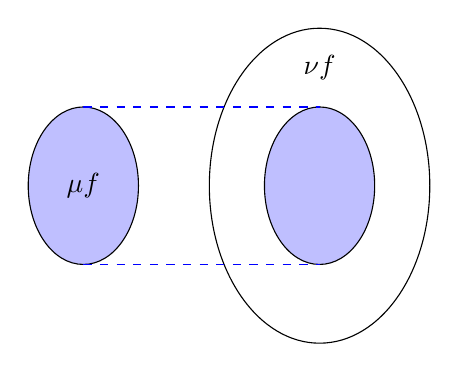
\begin{tikzpicture}
         \draw (-1,0)[fill=blue!25!white] ellipse (0.7 and 1);
         \draw (2,0) ellipse (1.4 and 2);
         \draw (2,0)[fill=blue!25!white] ellipse (0.7 and 1);
       	\draw[dashed, blue] (-1, 1) -- (2, 1);
	\draw[dashed, blue] (-1, -1) -- (2, -1);
        \node at (-1, 0) { $\mu f$ };
        \node at (2, 1.5) { $\nu f$ };
\end{tikzpicture}
\end{figure}

It turns out that \hask{fromNuToMu} is its inverse, proving that, in Haskell (but \emph{not} in $Set$), these two fixed points are isomorphic.

The fact that, in Haskell, we can map a terminal coalgebra to an initial algebra is the reason why we have hylomorphisms. A hylomorphism uses a coalgebra to build a recursive data structure from a seed, and then applies an algebra to fold it. It applies a catamorphism to the result of an anamorphism, which is only possible because they have the same type in the middle. 

\begin{figure}[H]
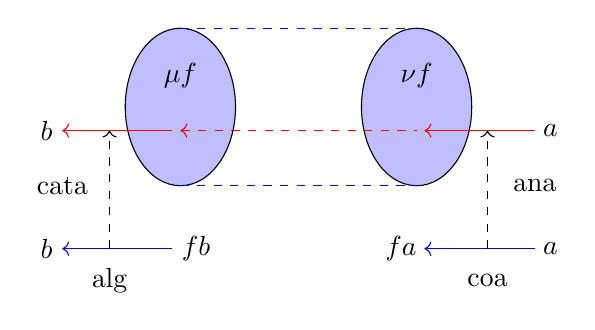
\begin{tikzpicture}
         \draw (-1.5,0)[fill=blue!25!white] ellipse (0.7 and 1);
         \draw ( 1.5,0)[fill=blue!25!white] ellipse (0.7 and 1);
       	\draw[dashed, blue] (-1.5,  1) -- (1.5,  1);
	\draw[dashed, blue] (-1.5, -1) -- (1.5, -1);
        \node at (-1.5, 0.4) { $\mu f$ };
        \node at ( 1.5, 0.4) { $\nu f$ };
	\draw[<-, red, dashed] (-1.5, -0.3) -- (1.5, -0.3);
	\draw[<-, red] (-3, -0.3) -- (-1.6, -0.3);
	\draw[<-, red] ( 1.6, -0.3) -- ( 3.0, -0.3);
        \node at (-3.2, -0.3) { $b$ };
        \node at (3.2, -0.3) { $a$ };
	\draw[<-, blue] (-3.0, -1.8) -- (-1.6, -1.8);
	\draw[<-, blue] (1.6, -1.8) -- (3.0, -1.8);
        \node at (-3.2, -1.8) { $b$ };
        \node at (3.2, -1.8) { $a$ };
        \node at (-1.3, -1.8) { $f b$ };
        \node at (1.3, -1.8) { $f a$ };
        \draw[->, dashed] ( 2.4, -1.8) -- ( 2.4, -0.3);
        \draw[->, dashed] (-2.4, -1.8) -- (-2.4, -0.3);
        \node at (-3, -1) { cata };
        \node at ( 3, -1) { ana };
        \node at (-2.4, -2.2) { alg };
        \node at ( 2.4, -2.2) { coa };
\end{tikzpicture}
\caption{A hylomorphism (in red), assuming that $\mu f$ is isomorphic to $\nu f$}
\end{figure}

Here's a quick exercise that was hinted at in the previous installment. This is a tree functor
\begin{haskell}
data TreeF a x = LeafF | NodeF a x x
  deriving Functor
\end{haskell}
We define a coalgebra that uses a list of \hask{a} as a seed, and partitions this list between its two children, storing the pivot at the node
\begin{haskell}
split :: Ord a => Coalgebra (TreeF a) [a]
split [] = LeafF
split (a : as) = NodeF a l r
  where (l, r) = partition (<a) as
\end{haskell}
Here's the algebra that concatenates child lists with the pivot in between
\begin{haskell}
combine :: Algebra (TreeF Int) [Int]
combine LeafF = []
combine (NodeF a b c) = b ++ [a] ++ c
\end{haskell}
And this is quicksort implemented using functions defined in this section
\begin{haskell}
qsort = cataMu combine . fromNuToMu . anaNu split
\end{haskell}
This is an example of a hylomorphism. The actual implementation of a hylomorphism in the Haskell library is more efficient, as it fuses the the recursive functions
\begin{haskell}
hylo :: Functor f => Algebra f a -> Coalgebra f b -> b -> a
hylo alg coa = alg . fmap (hylo alg coa) . coa
\end{haskell}

\section{End/Coend formulation}

Let's rewrite \hask{Mu} using GADTs
\begin{haskell}
data Mu f where
  Mu :: (forall a. (f a -> a) -> a) -> Mu f
\end{haskell}
In category theory, this is called an end
\[\mu f = \int_a a^{C(f a, a)}\]
In general an end over a profunctor \hask{p a b} is defined in Haskell as
\begin{haskell}
data End p where
  End :: (forall a. p a a) -> End p
\end{haskell}
Here, the profunctor is
\[p a b = b^{ C(f b, a)}\]
where $a$ and $b$ are objects in the category $C$ and $C(f b, a)$ is the hom-set (the set of morphisms) from $f b$ to $a$. In Haskell, we would write it as
\begin{haskell}
data P f a b = P ((f b -> a) -> b)
\end{haskell}
A profunctor is covariant in its second argument and contravariant in the first
\begin{haskell}
instance Functor f => Profunctor (P f) where
  dimap g g' (P h) = P (\j -> g'( h (g . j . fmap g')))
\end{haskell}

The Haskell function type from \hask{(f b -> a)} to \hask{b} is represented in category theory as a \emph{power}
\[b^{ C(f b, a)}\]
We have to use a power because $b$ is an object whereas $C(f b, a)$ is a set. The power is defined by the isomorphism
\[ C(x, a^s) \cong Set(s, C(x, a)) \]
The end behaves like a gigantic product in the sense that it defines projections $\pi_a$ for every $a$. In our case, these projections are the catamorphisms
\[\pi_a \colon \mu f \to a^{C(f a, a)}\]
Indeed, such a projection is a member of the hom-set
\[C(\mu f, a^{C(f a, a)})\]
By the definition of the power, it corresponds to an element of the set
\[Set(C(f a, a), C(\mu f, a))\]
which maps algebras, members of $C(f a, a)$, to mappings out of the initial algebra, $C(\mu f, a)$. These are the catamorphisms.

Similarly, we can rewrite \hask{Nu}
\begin{haskell}
data Nu f where 
  Nu :: (a -> f a) -> a -> Nu f
\end{haskell}
as a coend
\[\nu f = \int^a C(a, f a) \cdot a \]
over the profunctor
\[q a b = C(a, f b) \cdot b\]
where the dot is the copower, defined by the isomorphism
\[ C(s \cdot a, x) \cong Set(s, C(a, x))\]

In Haskell, this profunctor would be defined as
\begin{haskell}
data Q f a b = Q (a -> f b) b
\end{haskell}

\begin{haskell}
instance Functor f => Profunctor (Q f) where
  dimap g g' (Q h b) = Q (fmap g' . h . g) (g' b)
\end{haskell}
and the coend is an existential data type defined using a GADT
\begin{haskell}
data Coend p where
  Coend :: p a a -> Coend p
\end{haskell}


A coend behaves like a gigantic sum, in the sense that it defines injections $\iota_a$ for every $a$. In our case, these injections are anamorphisms
\[ \iota_a \colon C(a, f a) \cdot a \to \nu f\]
Indeed $\iota_a$ is a member of the hom-set
\[C(C(a, f a) \cdot a, \nu f)\]
or, using the definition of the copower, an element of the set
\[Set(C(a, f a), C(a, \nu f))\]
which we recognize as an anamorphism.

\section{Hylomorphism categorically}

If the mapping from from the terminal coalgebra $\nu$ to the initial algebra $\mu$ exists in a particular category $C$, it is an element of the following hom-set

\[C \Big(\int^a C(a, f a) \cdot a, \int_b b^{C(f b, b)} \Big)\]

We'll apply some coend-fu to transform it into a more familiar form. 

We use the co-continuity of the hom-functor to move the coend out of the left side of the hom-set. It becomes an end in the process

\[ \int_a C \Big( C(a, f a) \cdot a, \int_b b^{C(f b, b)}\Big)\]

Using continuity we move the end out of the right side of the hom-set

\[ \int_{a, b} C \Big( C(a, f a) \cdot a, b^{C(f b, b)}\Big)\]

Using the definition of the copower
\[ C(s \cdot a, x) \cong Set(s, C(a, x))\]
we get
\[ \int_{a, b} Set \Big(C(a, f a), C(a, b^{C(f b, b)})\Big)\]
And using the definition of the power
\[ C(x, a^s) \cong Set(s, C(x, a)) \]
we get
\[ \int_{a, b} Set \Big(C(a, f a), Set\big(C(f b, b), C(a, b)\big)\Big)\]
Finally, applying the currying adjunction in $Set$ we get
\[ \int_{a, b} Set \Big(C(a, f a) \times C(f b, b), C(a, b)\Big)\]
which has the form reminiscent of the Haskell definition of a hylomorphism

\begin{haskell}
hylo :: Functor f => Coalgebra f a -> Algebra f b -> a -> b
hylo coa alg = alg . fmap (hylo coa alg) . coa
\end{haskell}
This makes sense in Haskell even though it won't work in Set, because Haskell is okay with non-terminating recursion. 

I had a discussion with Derek Elkins, who pointed me to the paper by Fokkinga and Meijer, in which they discuss the existence of hylomorphisms in CPOs. 

\section{bibliography}
\begin{itemize}
\item Fosco Loregian, \href{https://arxiv.org/abs/1501.02503}{Coend calculus}
\item Fokkinga, Meijer, \href{https://maartenfokkinga.github.io/utwente/mmf91a.pdf}{Program Calculation Properties of Continuous Algebras}
\end{itemize}
\end{document}


